\documentclass[twocolumn, 11pt]{article}%
\usepackage{amsmath, amssymb, esint, gensymb, enumitem}
\usepackage{graphicx, cuted, geometry, float, chemfig}

\geometry{
    a4paper,
    total={170mm,260mm},
}

\begin{document}

\begin{strip}
  \vspace*{\dimexpr-\stripsep}
  \begin{center}
      \Large\textbf{FISIKA III}\\
      \large{Minggu 1 (NO ABSEN)}\\
      \large{\today}\\
   \end{center}
\end{strip}

\section{Termometri dan Kalorimetri}
    \subsection{Konsep Temperatur}
        \paragraph{ } Temperatur adalah ukuran panas atau dinginnya suatu benda, bisa juga diartikan dengan ukuran \textbf{energi kinetik molekular internal rata-rata suatu benda.}

        Energi termal adalah energi total semua molekul suatu benda. Dan panas adalah transfer energi dari suatu benda ke benda lain karena perbedaan temperatur (beda dengan energi termal), jadi panas adalah relatif tergantung selisih perbedaan temperatur.\\

        \textbf{Contoh :}

        50 gram air $30\degree C$ dicampur dengan 200 gram air $25\degree C$, terjadi aliran panas dari air $30\degree C$ ke $25\degree C$ walaupun air $25\degree C$ mempunyai energi termal yang lebih besar (karena memiliki massa yang lebih besar). Temperatur akhir campuran terjadi apabila telah tercapai \textbf{kesetimbangan termal.}

        \subsubsection{Hukum Ke-0 Termodinamika (Hukum Keseimbangan)}
        Jika objek A dan B terpisah dalam kesetimbangan termal dengan objek C, maka A dan B berada pada kesetimbangan termal dengan satu sama lain.

        \begin{center}
            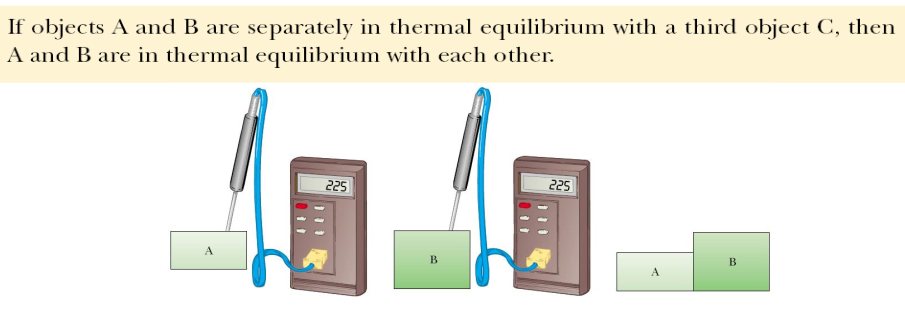
\includegraphics[width=235px]{1.png}
        \end{center}

        \subsubsection{Ukuran Kualitatif temperatur}
        Biasa disebut dingin, panas, hangat, dsb. Ukuran kualitatif tersebut dicari dengan memanfaatkan \textbf{sifat termometris} benda (sifat fisis yang berubah karena perubahan temperatur) seperti hambatan listrik, padatan dan yang memuai, tekanan gas pada volume tetap, volume gas pada tekanan tetap, warna kawat pijar, dsb.

    \subsection{Pengukuran Temperatur (Termometer)}
        Temperatur pada nilai tertentu adalah
        \[T(x) = ax \]
        \textbf{Dimana:}

        $x=$ Sifat Termometris
        
        $a=$ Konstanta (tergantung jenis bahan)

        Jika dijadikan formula perbandingan menjadi seperti berikut
        \begin{equation*}
            \begin{split}
                \frac{T(x)}{T(x_s)} &= \frac{ax}{ax_s}\\\\
                T(x) &= T(x_s) \frac{x}{x_s}
            \end{split}
        \end{equation*}

        Untuk menera termometer digunakan titik standar yang tetap yaitu titik tripel air
        $$[T(x_s) = 273.16\ K\ (kelvin)]$$
        $$ T(x) = (273.16\ K) \frac{x}{x_s}$$

        Titik tripel air bisa digambar dalam grafik diagram fasa sebagai berikut

        \begin{center}
            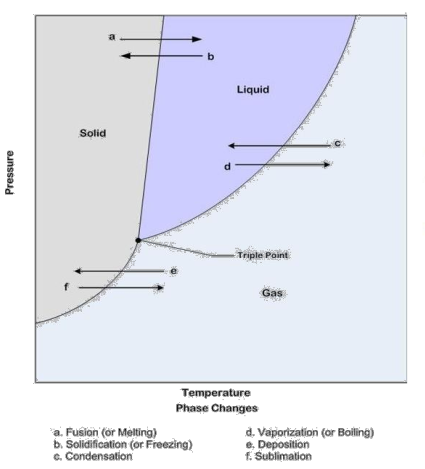
\includegraphics[width=235px]{2.png}
        \end{center}

        \textbf{Contoh:}

        Sebuah termometer hambatan (platina) mempunyai hambatan R sebesar $90,35\ \Omega$ bila pentolan (bulb) termometer ditempatkan di dalam sebuah sel titik tripel. Berapakah harga temperaturnya jika pentolan tersebut ditempatkan di dalam sebuah lingkungan hingga hambatannya berharga $96,28\ \Omega$ ?
        
        \textbf{Penyelesaian:}

        Sifat termometris termometer ini berupa hambatan listrik.

        \begin{equation*}
            \begin{split}
                T(x) &= (273.16\ K)\ \frac{x}{x_s}\\
                T(x) &= (273.16\ K)\ \frac{96.28 \Omega}{90.35 \Omega}\\
                T(x) &= 280.6 K
            \end{split}
        \end{equation*}

    \subsection{Skala Temperatur}
        \begin{center}
            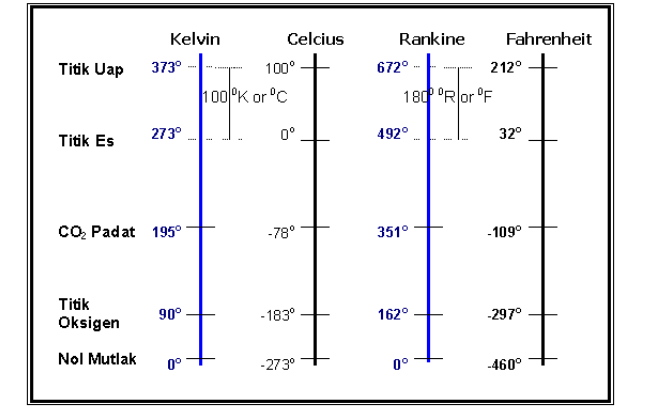
\includegraphics[width=230px]{3.png}
        \end{center}

        Dimana

        \begin{equation*}
            \begin{split}
                T_C &= T_K - 273.16\\
                T_R &= \frac{9}{5} T_K\\
                T_F &= T_R - 495,67\\
                T_F &= \frac{9}{5} T_C + 32
            \end{split}
        \end{equation*}

        \textbf{Contoh:}

        Titik lebur perak dalam skala Farenheit adalah $1760\ \degree F$. Nyatakan titik lebur tersebut dalam $\degree C$, $\degree K$, $\degree R$

        \textbf{Penyelesaian:}

        Pertama menentukan titik lebur perak pada skala Celcius.
        \begin{equation*}
            \begin{split}
                T_F &= \frac{9}{5} T_C + 32\\
                T_C &= \frac{5}{9} (T_F - 32)\\
                &= \frac{5}{9} (1760 - 32)\\
                &= 960\degree C
            \end{split}
        \end{equation*}

        Selanjutnya dapat dicari temperatur pada skala kelvin
        \begin{equation*}
            \begin{split}
                T_C &=T - 273.16\\
                T &= T_C + 273.16\\
                &= 1233.16 K
            \end{split}
        \end{equation*}

        Untuk memperoleh temperatur dalam skala Rankine dapat diperoleh langsung dari skala Farenheit sebagai berikut
        \begin{equation*}
            \begin{split}
                T_F &=T_R - 459.67\\
                T_R &= T_F + 459.67\\
                &= 1760 + 459.67\\
                &= 2219,67 \degree R
            \end{split}
        \end{equation*}

        \subsection{Pemuaian}
        Pemuaian terbagi menjadi beberapa jenis dengan rumus yang berbeda-beda.\\
        
        \textbf{Perubahan panjang karena perubahan temperatur:}

        \begin{equation*}
           \begin{split}
               \Delta L &= \alpha L \Delta T\\
               L &= L_0 (1+\alpha \Delta T)\\
           \end{split} 
        \end{equation*}
        Dimana $\alpha$ adalah koefisien muai panjang (tergantung material).

        \textbf{Perubahan Luasan karena perubahan temperatur:}

        \begin{equation*}
           \begin{split}
               \Delta A &= \gamma A \Delta T\\
               A &= A_0 (1+ \gamma \Delta T)
           \end{split} 
        \end{equation*}

        dimana $\gamma$ adalah \textbf{koefisien muai luas} dan\\
        $\gamma = 2 \alpha$.

        \textbf{Perubahan volume karena perubahan temperatur:}

        \begin{equation*}
            \begin{split}
                \Delta V &= \beta L \Delta T \\
                V &= V_0 (1+ \beta \Delta T)
           \end{split} 
        \end{equation*}

        dimana $\beta$ adalah koefisien muai volume/ruang dan $\beta = 3 \alpha$.

        Aplikasi dari pemuaian adalah Bimetal dimana ada 2 logam yang dibuat berlapis, karena perbedaan koefisien muai panjang, maka jika ada perubahan temperatur, lempengan logam tersebut akan melengkung.

        \begin{center}
            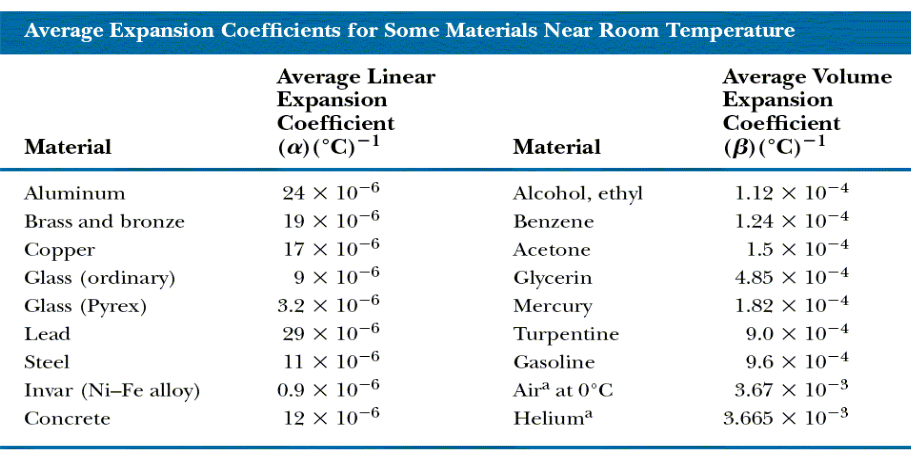
\includegraphics[width=250px]{4.png}
        \end{center}

        \textbf{Contoh:}

        Volume bola termometer air raksa dalam gelas pada $0\degree C$ adalah 0.15 $cm^3$, sedangkan luas penampang tabungnya $10^{-3} m^2$. Koefisien muai panjang gelas adalah $5\times10^{-6}\ \degree C^{-1}$, sedangkan koefisien muai ruang air raksa $0.182 \times 10^{-3}\ degree C^{-1}$. Kalau pada $0\degree C$ air raksa tepat memenuhi seluruh bola, berapa tinggi kolom air raksa pada temperatur $100 \degree C$ ?

        \textbf{Penyelesaian:}

        Volume air raksa pada $100 \degree C$:
        \begin{equation*}
            \begin{split}
                V_{Hg} &= V_0 (1+ \beta \Delta T)\\
                &= 0.15\ cm^3\ (1+ 0.182 \times 10^{-3} \times 100)\\
                &= 0.15273\ cm^3
            \end{split}
        \end{equation*}
        
        Volume bola pada $100 \degree C$:
        \begin{equation*}
            \begin{split}
                V_{bola} &= V_0 (1+ 3\alpha_{gelas} \Delta T)\\
                &= 0.15\ cm^3\ (1+ 3 \times 5 \times 10^{-6} \times 100)\\
                &= 0.150225\ cm^3
            \end{split}
        \end{equation*}
        
        Volume air raksa yang keluar dari bola pada $100 \degree C$:
        \begin{equation*}
            V_{Hg} - V_{bola} = 2.5 \times 10^{-3}\ cm^3
        \end{equation*}

        Luas penampang tabung pada $100 \degree C$:
        \begin{equation*}
            \begin{split}
                A_{100} &= A_0 (1+2\alpha \Delta T)\\
                &= 10^{-3} cm^2
            \end{split}
        \end{equation*}

        Sehingga tinggi kolom air raksa adalah:
        \begin{equation*}
            \begin{split}
                h &= \frac{V_{Hg} - V_{bola}}{A_{100}}\\
                &= \frac{2.5 \times \textperthousand{10}\ cm^{-3}}{10^{-3}\ cm^{-2}}\\
                &= 2.5\ cm
            \end{split}
        \end{equation*}

        \subsection{Konsep Panas dan Perubahan Fase}
        \textbf{Kapasitas Panas:}

        Jumlah panas yang diperlukan untuk menaikkan temperatur sebanyak $1\degree C$.

        \[ C = \frac{dQ}{dT} \]

        \textbf{Kapasitas Panas Jenis:}
        
        Kapasitas panas benda 1 gram
        \[c= \frac{dQ}{m\ dT} \]

        Jika c konstan, maka
        \[ Q=mc \Delta T \]

        \textbf{Kuantitas Panas Q:}

        Jumlah energi yang dipindahkan dalam kurun waktu tertentu. Satuan Q adalah \textbf{kalori, joule, BTU (British Termal Unit)}.

        Definisi \textbf{1 kalori} adalah jumlah panas yang diperlukan untuk menaikkan temperatur 1 gram air sebesar $1\degree C$, misal dari temperatur $14.5\degree C$ menjadi $15.5\degree C$ pada tekanan 1 atm.

        \begin{itemize}
                \item 1 kalori = 4.186 Joule
                \item 1 BTU = 251.996 kalori
        \end{itemize}

        Dulu, tepatnya pada abad ke-18, panas dimodelkan sebagai gerakan material dan fluida (caloric). Namun \textbf{sekarang, panas dimodelkan sebagai kerja dan energi.}\\
        
        \textbf{Perubahan Fase}

        \begin{center}
            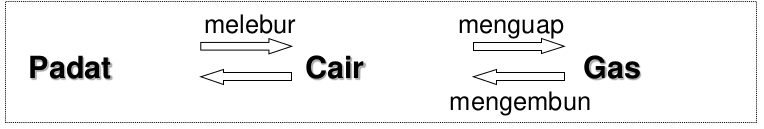
\includegraphics[width=230px]{5.png}
        \end{center}

        Kuantitas panas pada perubahan fase ialah
        \[ Q=mL \]
        dimana L adalah panas laten.
        \begin{center}
            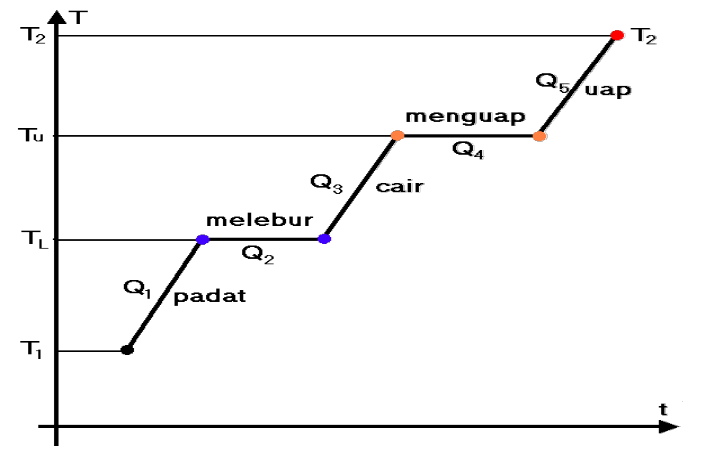
\includegraphics[width=230px]{6.png}
        \end{center}

        \textbf{Asas Black}

        \textit{"Panas yang dilepas sama dengan panas yang diterima"}
        \[Q_1 = Q_2 \]

        \begin{center}
            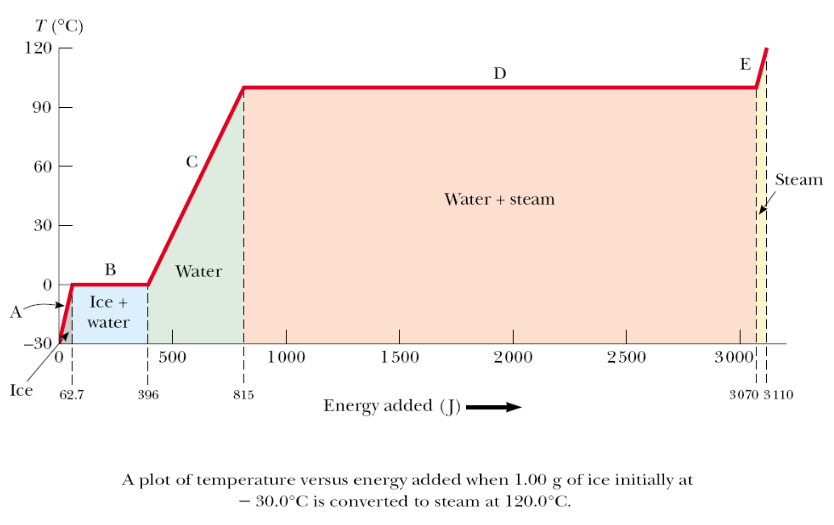
\includegraphics[width=230px]{7.png}
        \end{center}

        \textbf{Contoh:}

        Suatu bejana berisi 1 kg es dengan temperatur $-10\degree C$. Kapasitas panas bejana dapat diabaikan. Kepada sistem diberi panas rata-rata 2000 kal/menit selama 100 menit.
        \begin{enumerate}[label=\alph*)]
            \item Buatlah diagram fase yang menyatakan hubungan antara temperatur dan waktu, dari es tersebut!
            \item Berapa banyaknya es yang menguap?
        \end{enumerate}

        \textbf{\underline{Penyelesaian}}
        \begin{enumerate}[label=\alph*)]
            \item 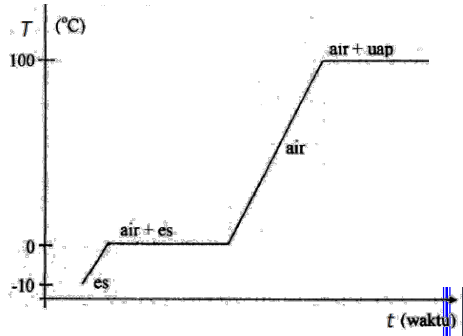
\includegraphics[width=190px]{8.png}
            \item Jumlah panas yang diberikan\\
                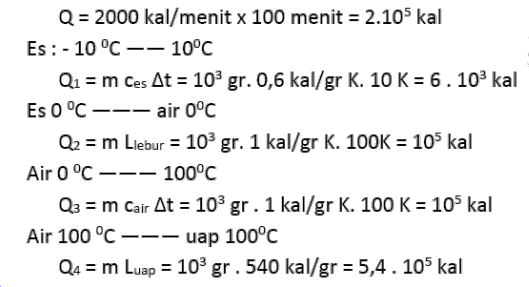
\includegraphics[width=220px]{9.png}
                Jika semua es berubah menjadi uap, maka panas yang dibutuhkan adalah:
                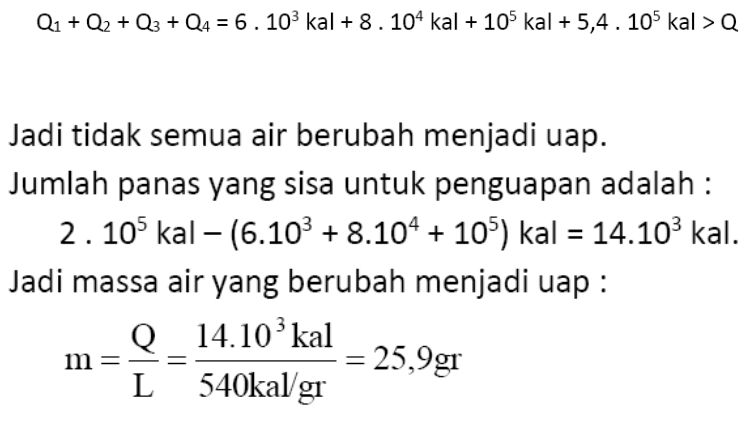
\includegraphics[width=220px]{10.png}
        \end{enumerate}

    \subsection{Kalorimeter}
        Kalorimeter adalah alat untuk menentukan kapasitas panas suatu zat.
        
        \begin{center}
            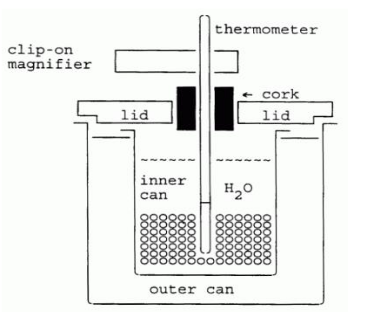
\includegraphics[width=150px]{11.png}
            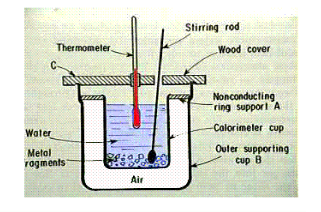
\includegraphics[width=220px]{12.png}
            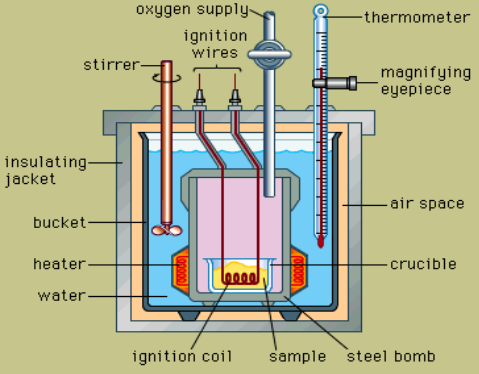
\includegraphics[width=220px]{13.png}
            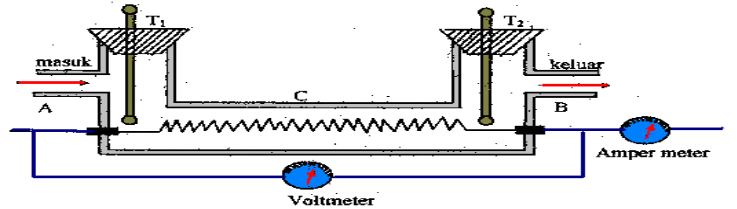
\includegraphics[width=220px]{14.png}
        \end{center}

\end{document}
